% Report metadata.
\renewcommand{\labCourse}{P4}
\renewcommand{\groupNumber}{}
\renewcommand{\groupDay}{}
% Match the marker position to the selected group day.
\renewcommand{\groupDayPosition}{}
%\renewcommand{\groupDayPosition}{11.7cm,22.8cm} % Mo2
%\renewcommand{\groupDayPosition}{13.3cm,22.8cm} % Mi3
\renewcommand{\term}{}
\renewcommand{\experimentName}{}
\renewcommand{\studentOneName}{}
\renewcommand{\studentOneEmail}{}
\renewcommand{\studentTwoName}{}
\renewcommand{\studentTwoEmail}{}
\renewcommand{\supervisorName}{}
\renewcommand{\experimentDate}{}
\renewcommand{\submissionDate}{}
\begin{tikzpicture}[remember picture,overlay]
    \node at (current page.center) {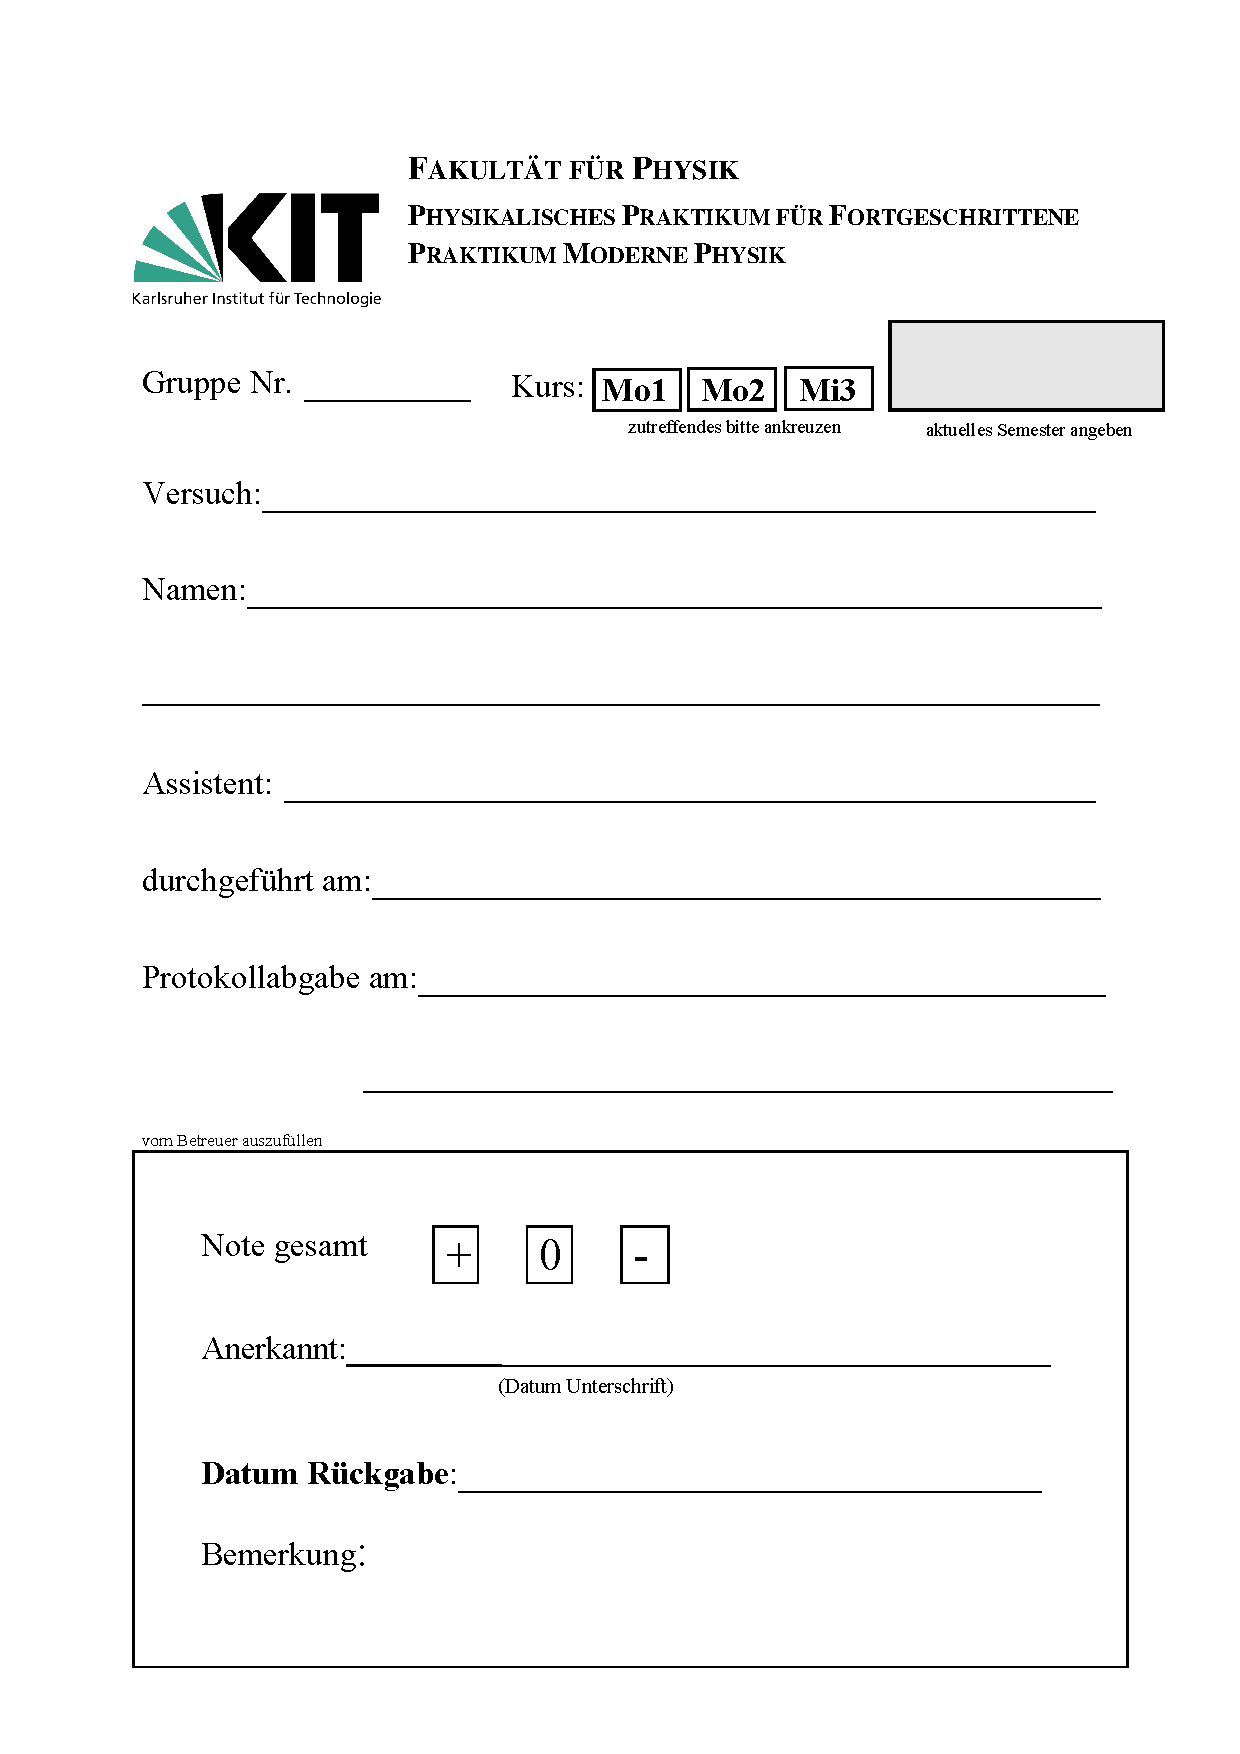
\includegraphics[page=1]{include/cover-page.pdf}};
    \begin{scope}[shift={(current page.south west)},every node/.style={anchor=base west}]
        \node at (5.8cm,23.1cm){\Large{\groupNumber}};
        \ifx\groupDayPosition\empty\else
          \node at (\groupDayPosition) {\scalebox{4}{{$\mathbf{\times}$}}};
        \fi
        \node at (16cm,23.1cm) {\Large{\term}};
        \node at (4.8cm,21.2cm){\Large{\experimentName}};
        \node at (4.8cm,19.6cm){\Large{\studentOneName\hspace{0.2222em}(\studentOneEmail)}};
        \node at (4.8cm,18.0cm){\Large{\studentTwoName\hspace{0.2222em}(\studentTwoEmail)}};
        \node at (4.8cm,16.3cm){\Large{\supervisorName}};
        \node at (7.2cm,14.6cm){\Large{\experimentDate}};
        \node at (7.2cm,13.0cm){\Large{\submissionDate}};
    \end{scope}
\end{tikzpicture}
\hypersetup{
  pdftitle    = {\labCourse\hspace{0.2222em}Lab Report - \experimentName},
  pdfsubject  = {Report for experiment \experimentName\hspace{0.2222em}on \experimentDate},
  pdfauthor   = {KIT Physics Laboratory},
  pdfkeywords = {KIT, Physics, Laboratory, Lab Report, \labCourse, \experimentName},
  pdfcreator  = {pdflatex},
  pdfproducer = {LaTeX with hyperref}
}